\documentclass[a4paper]{article}
\usepackage[utf8]{inputenc}
\usepackage[T1]{fontenc}
\usepackage[pdftex]{graphicx}
\usepackage{fancyhdr}
\usepackage{lscape}
\usepackage{color}
\usepackage{qtree}
\usepackage[english]{babel}
\usepackage{graphicx}
\usepackage[colorinlistoftodos]{todonotes}
\usepackage{listings}
\usepackage{color}
\usepackage{changepage}
\usepackage[margin=1in]{geometry}
\definecolor{codegreen}{rgb}{0,0.6,0}
\definecolor{codegray}{rgb}{0.5,0.5,0.5}
\definecolor{codepurple}{rgb}{0.58,0,0.82}
\definecolor{backcolour}{rgb}{0.95,0.95,0.92}
\usepackage[parfill]{parskip}

 \lstdefinestyle{mystyle}{
 	backgroundcolor=\color{backcolour},   
 	commentstyle=\color{codegreen},
 	keywordstyle=\color{magenta},
 	numberstyle=\tiny\color{codegray},
 	stringstyle=\color{codepurple},
 	basicstyle=\footnotesize,
 	breakatwhitespace=false,         
 	breaklines=true,                 
 	captionpos=b,                    
 	keepspaces=true,                 
 	numbers=left,                    
 	numbersep=5pt,                  
 	showspaces=false,                
 	showstringspaces=false,
 	showtabs=false,                  
 	tabsize=2
 }
 
\lstset{
	style=mystyle,
	inputencoding=utf8,
	extendedchars=true,
	literate={á}{{\'a}}1 {ã}{{\~a}}1 {é}{{\'e}}1,
	escapechar=\&
}
\title{Algorithmique et structures de données : Mission 2}
\date{30 octobre 2014}
\author{Groupe 1.2: Ivan Ahad - Jérôme Bertaux - Rodolphe Cambier \\ 
	Baptiste Degryse - Wojciech Grynczel - Charles Jaquet}



\begin{document}
\maketitle



Rapport écrit par Ivan Ahad, Rodolphe Cambier et Charles Jacquet

\subsection*{Introduction}
Pour ce programme, nous avions à implémenter une map pour contenir les information sur le classement de magasines. Chaque magasine contient plusieurs informations, comme son nom (qui le distingue des autres), sa note, etc ... .
Nous allons commencer par présenter le fonctionnement de notre programme, ensuite nous parlerons le l'évaluation des performance de celui-ci. Et nous terminerons par les tests que nous avons effectué.

\subsection*{Choix d'implémentations et fonctionnement}
Le main commence par créer un nouveau "Journal".Ensuite, fait une boucle dans laquelle il demande à l'utilisateur un nom de journal à rechercher.
Et recommence ces deux dernières opération tant que l'utisateur ne veuille plus continuer.
Pour ce qui est de la classe Journal. le constructeur prends plusieurs arguments. Le premier est l'index de la clé qui sera utilisée (c'est à dire, pour nous le nom avec l'index 1). Le deuxième est le nom du fichier et enfin le dernier est le délimiteur utilisé.\\
Fonctionnement du constructeur du journal:\\
Pour chaque ligne, il va faire un split avec le délimiteur rentré en argument. Ensuite, il va tester le nombre d'élements.S'il y en a pas suffisamment, alors il rajoute un tableau vide à la fin car ça signifie qu'il n'y a rien après les délimiteurs. S'il y en a de trop, il check les guillemets pour remettre ensemble les tableaux qui ne devait pas être séparé. Enfin Il rajoute l'élément à une map, déjà implémentée en java. Pour le rajout d'un élément, il utilise également la classe Entrée qui permet de lier les clés et les valeurs ensemble.

\section*{Evaluation des performances}

\section*{Les tests}



\subsection*{UML}
Attention inclure l'uml
%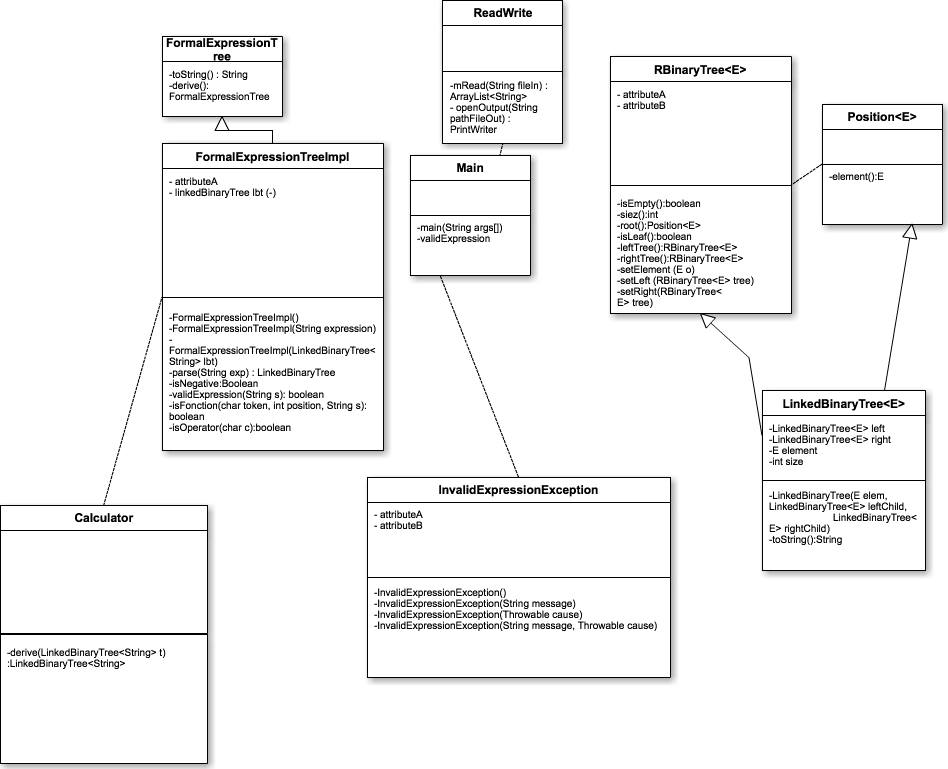
\includegraphics[scale=0.5]{uml}

\end{document}